\begin{comment}
\begin{figure}
\centering
%\includegraphics[width=.49\linewidth]{figures/xxxxxxx}
%\includegraphics[width=.49\linewidth]{figures/xxxxxxx}
%\includegraphics[width=.49\linewidth]{figures/xxxxxxx}
 \caption{Top left: azimuthal correlation distribution between D meson from b-hadron decay and charged particles obtained from a Monte Carlo simulation
based on Pythia (Perugia-0 tune) fitted with a 2+1 Gaussian + constant function. The violet histogram is the template obtained by scaling the baseline
in order to match that measured in data. Top right: data correlation distributions obtained after the subtraction of the feed-down component, using 3 different values of $f_{\rm prompt}$ resulting
from the variation of the charm and beauty quark masses and factorization and renormalization scales employed in the FONLL calculation. Bottom: ratios between the azimuthal
distribution obtained with the maximum and minimum $f_{\rm prompt}$ values and that obtained with the central $f_{\rm prompt}$ value.}
 \label{fig:feeddownDescription}
\end{figure}
\end{comment}
%
%
The contribution of correlations of D meson from b-hadron decay is subtracted from the data correlation distributions as:
\begin{equation}
\tilde{C}_{\rm prompt~D}(\Delta\phi)=\frac{1}{f_{\rm prompt}}\left(\tilde{C}_{\rm inclusive}(\Delta\phi)-(1-f_{\rm prompt})\tilde{C}_{\rm feed-down}^{\rm MC~templ}(\Delta\phi) \right).
\label{eqFeedDown}
\end{equation}
In the above equation, $\tilde{C}_{\rm inclusive}(\Delta\phi)$ and $\tilde{C}_{\rm prompt~D}(\Delta\phi)$ are per-trigger azimuthal correlation distributions before and after
feed-down contribution subtraction, $f_{\rm prompt}$ is the fraction of prompt D meson and $\tilde{C}_{\rm feed-down}^{\rm MC~templ}$ is a template
of the azimuthal correlation distribution for the feed-down component obtained from home-made Monte Carlo simulation at generated level, using PYTHIA6 with Perugia2011 tune.
In order to avoid biases related to the different event multiplicity in real and simulated events, the correlation distribution was shifted to have its minimum coinciding with the baseline of the data azimuthal-correlation distribution before feed-down subtraction. %[THIS HELD FOR pp...]A difference smaller than 8\% was observed in the simulation between the baseline values of the azimuthal-correlation distributions for prompt and feed-down D mesons. Considering the typical values of $f_{\rm prompt}$, this difference results in a shift of the baseline of $\tilde{C}_{\rm prompt~D}(\Delta\phi$ of less than 1\%, negligible with respect to the other uncertainties affecting the measurement.

\begin{figure}
\centering
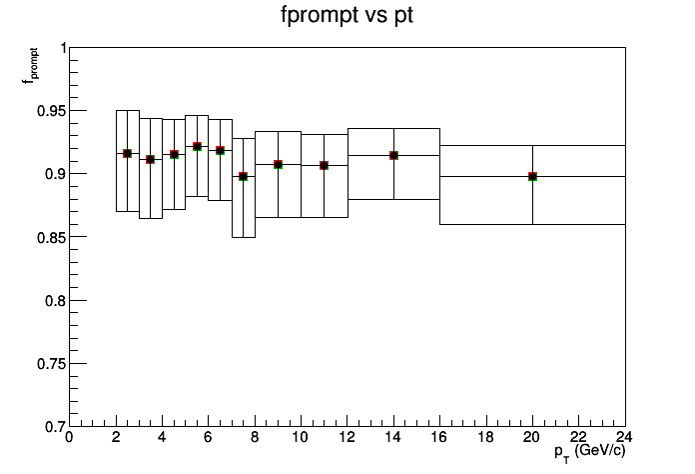
\includegraphics[width=0.6\linewidth]{figures/Effs/fprompt_D0.png}
\includegraphics[width=0.6\linewidth]{figures/Effs/fprompt_Dstar.png}
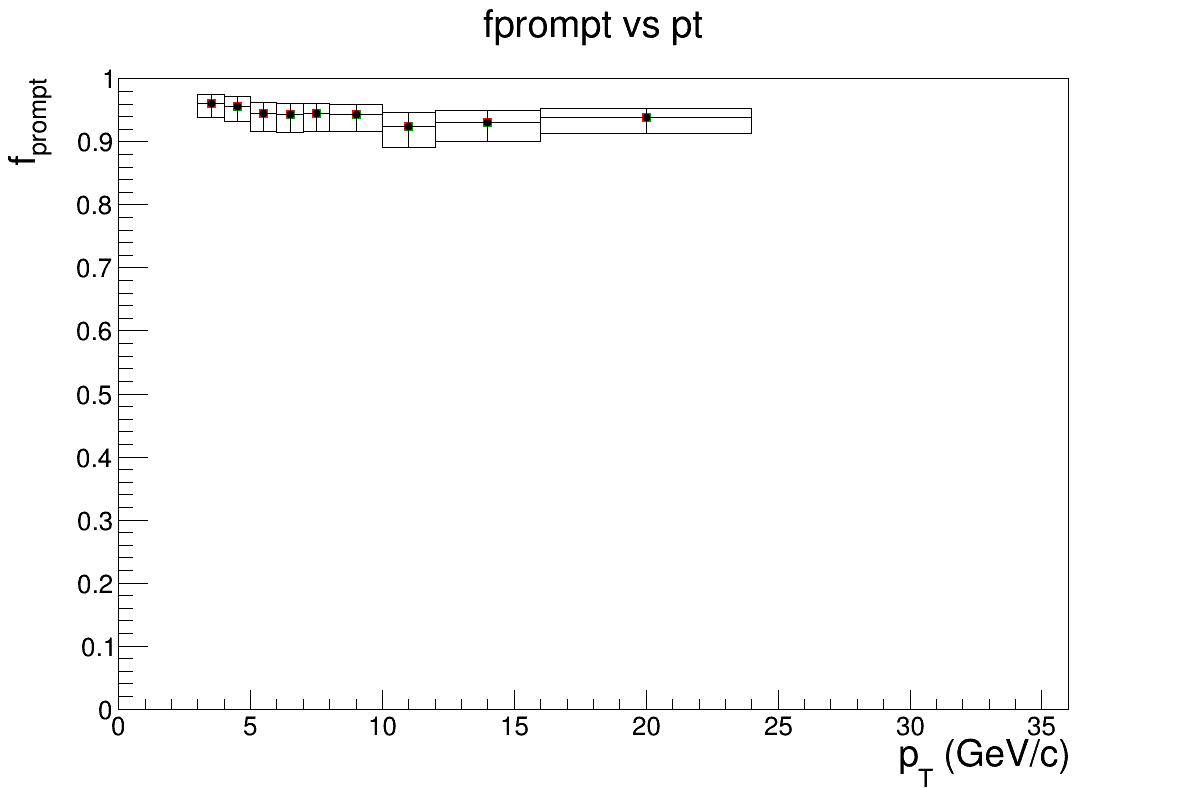
\includegraphics[width=0.6\linewidth]{figures/Effs/fpromptDplus.png}
\caption{$f_{\rm prompt}$ as a function of the $\pt$ for $\Dzero$ (top), $\Dstar$ (mid) and $\Dplus$ (bottom) estimated on the basis of FONLL predictions}
\end{figure}


The value of $f_{\rm prompt}$, which depends on D-meson species and varies as a function of the $\pt$, is estimated on the basis of FONLL predictions for the production of feed-down D mesons at central rapidity, in pp collisions at $\sqrt(s) = 5$ TeV, and using the reconstruction efficiency of prompt and feed-down D mesons, following the so-called $N_{\rm b}$ approach defined in~\cite{ALICEDmespp7Tev}. Typical values ranges are about 8-10\% for the
$\Dzero$, about 5\% for the $\Dplus$ and {\bf XXXX} percent for the $\Dstar$. The procedure adopted is the same as what done in pp: however, in p--Pb, in order to consider a possible non-zero $v_{2}$-like modulation of the baseline, a range of $0<v_{2}<0.2$ values for tracks and for secondary D mesons is considered for the systematic uncerainty evaluation (using an hypothesis of 0 for both cases for central values).

SOME TEMPLATE PLOTS HAVE TO BE ADDED HERE


\begin{figure}
\centering
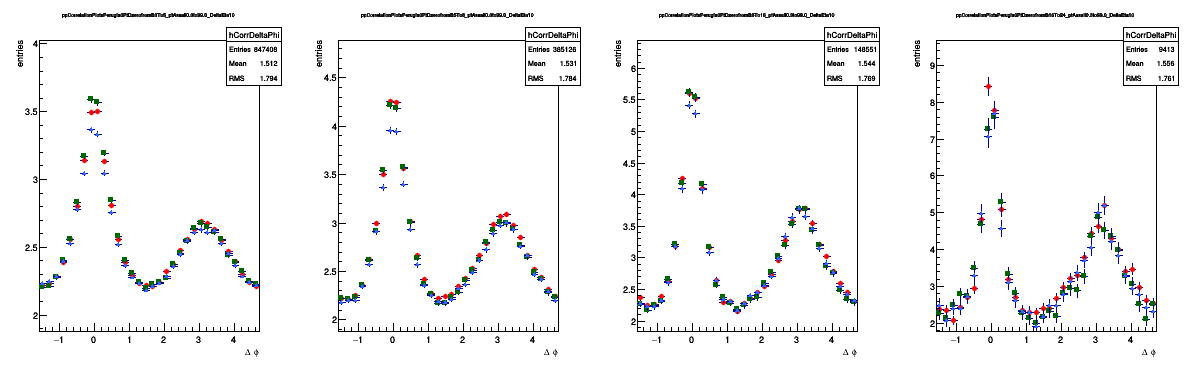
\includegraphics[width=1\linewidth]{figures/Template/1DCompare_allDpTfromB_AssoPt_0dot3to99dot0GeVc_Perugia0.png}
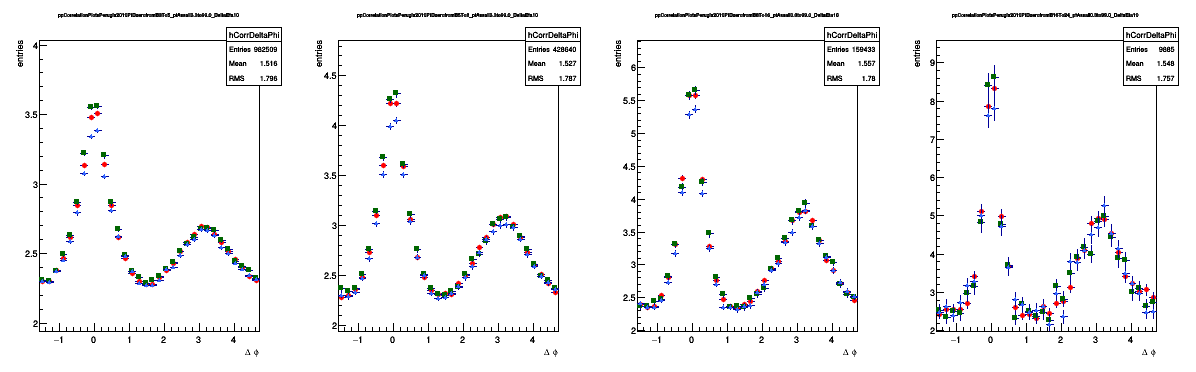
\includegraphics[width=1\linewidth]{figures/Template/1DCompare_allDpTfromB_AssoPt_0dot3to99dot0GeVc_Perugia2010.png}
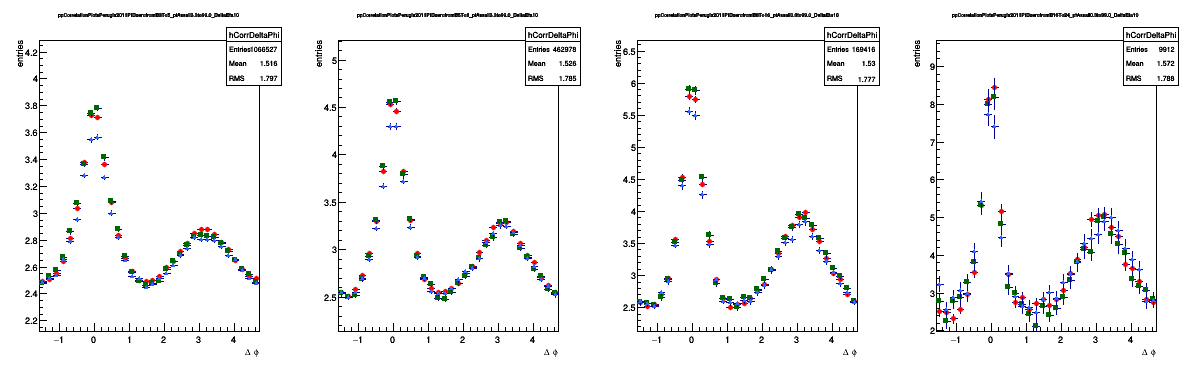
\includegraphics[width=1\linewidth]{figures/Template/1DCompare_allDpTfromB_AssoPt_0dot3to99dot0GeVc_Perugia2011.png}
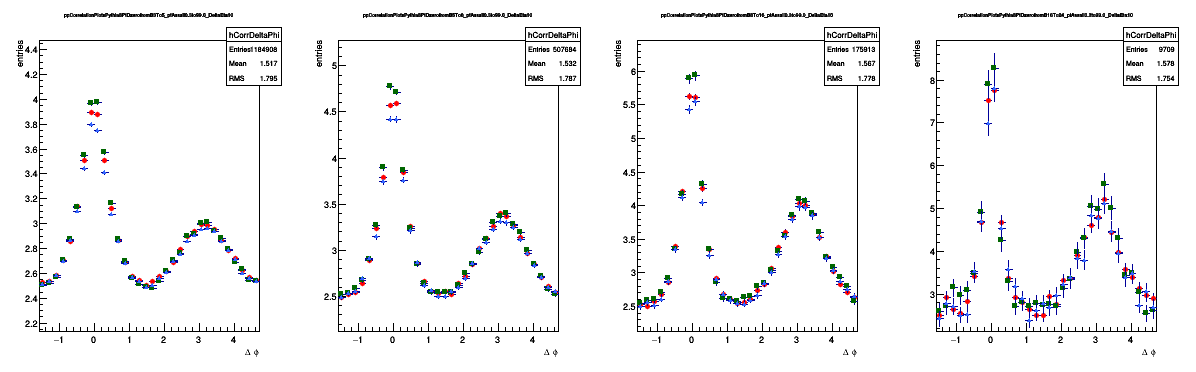
\includegraphics[width=1\linewidth]{figures/Template/1DCompare_allDpTfromB_AssoPt_0dot3to99dot0GeVc_Pythia8.png}
\caption{Top left: azimuthal correlation distribution between D meson from b-hadron decay and charged particles obtained from a Monte Carlo simulation
based on Pythia (Perugia-0 tune) fitted with a 2+1 Gaussian + constant function. The violet histogram is the template obtained by scaling the baseline
in order to match that measured in data. Top right: data correlation distributions obtained after the subtraction of the feed-down component, using 3 different values of $f_{\rm prompt}$ resulting
from the variation of the charm and beauty quark masses and factorization and renormalization scales employed in the FONLL calculation. Bottom: ratios between the azimuthal
distribution obtained with the maximum and minimum $f_{\rm prompt}$ values and that obtained with the central $f_{\rm prompt}$ value.}
\label{templates1}
\end{figure}

\begin{figure}
\centering
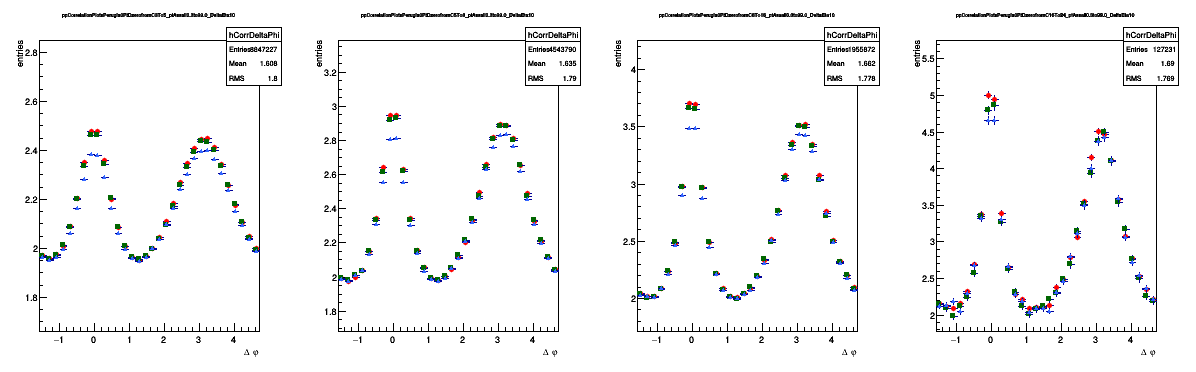
\includegraphics[width=1\linewidth]{figures/Template/1DCompare_allDpTfromC_AssoPt_0dot3to99dot0GeVc_Perugia0.png}
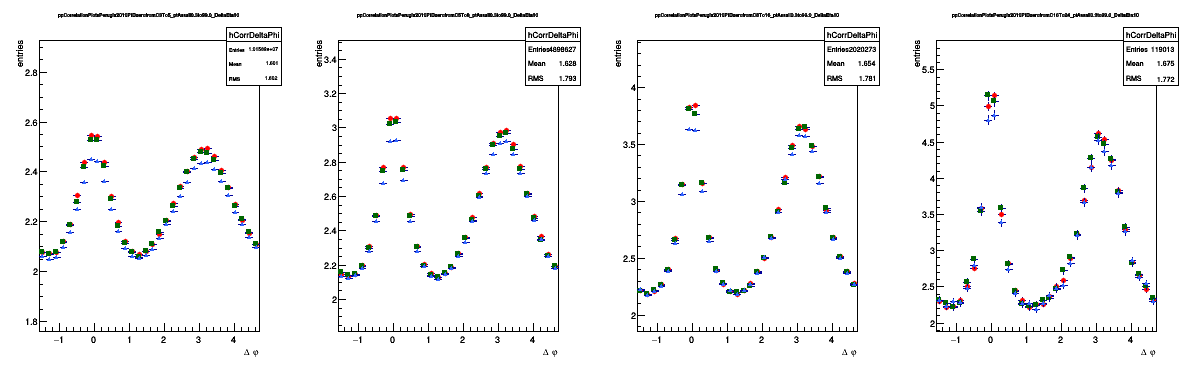
\includegraphics[width=1\linewidth]{figures/Template/1DCompare_allDpTfromC_AssoPt_0dot3to99dot0GeVc_Perugia2010.png}
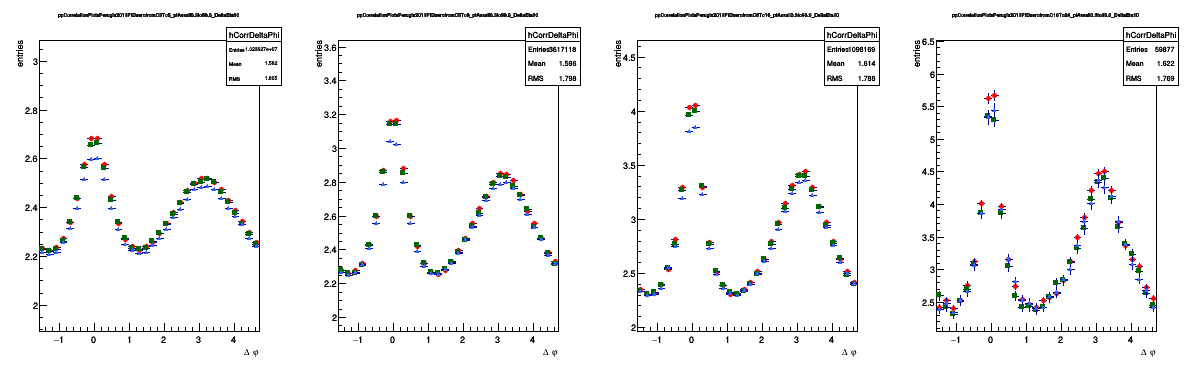
\includegraphics[width=1\linewidth]{figures/Template/1DCompare_allDpTfromC_AssoPt_0dot3to99dot0GeVc_Perugia2011.png}
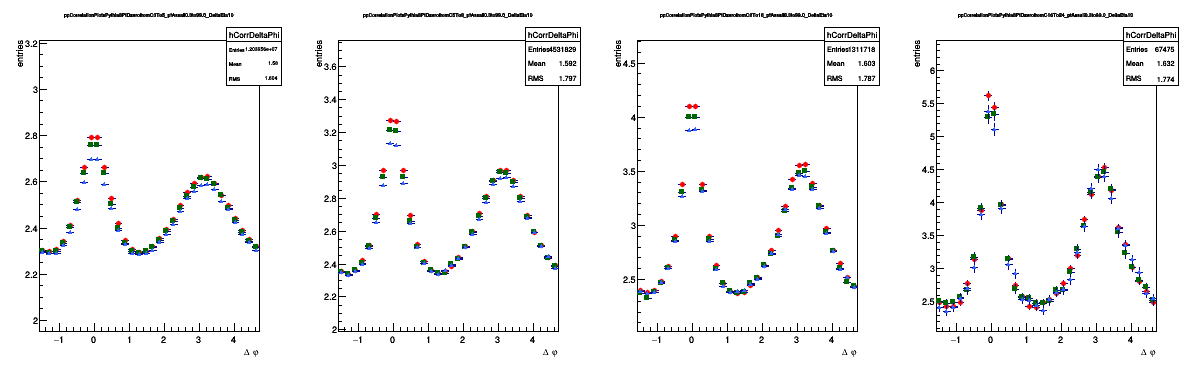
\includegraphics[width=1\linewidth]{figures/Template/1DCompare_allDpTfromC_AssoPt_0dot3to99dot0GeVc_Pythia8.png}
\caption{Top left: azimuthal correlation distribution between D meson from b-hadron decay and charged particles obtained from a Monte Carlo simulation
based on Pythia (Perugia-0 tune) fitted with a 2+1 Gaussian + constant function. The violet histogram is the template obtained by scaling the baseline
in order to match that measured in data. Top right: data correlation distributions obtained after the subtraction of the feed-down component, using 3 different values of $f_{\rm prompt}$ resulting
from the variation of the charm and beauty quark masses and factorization and renormalization scales employed in the FONLL calculation. Bottom: ratios between the azimuthal
distribution obtained with the maximum and minimum $f_{\rm prompt}$ values and that obtained with the central $f_{\rm prompt}$ value.}
\label{templates2}
\end{figure}

 %The green histogram in figure~\ref{fig:feeddownDescription}, top left panel, represents
%the azimuthal correlation distribution between D meson from b-hadron decay and charged particles obtained from a Monte Carlo simulation
%based on Pythia (Perugia-0 tune). This distribution is
%fitted with a function composed of 2 Gaussian, modeling the near-side peak, 1 Gaussian modeling the away-side peak and a constant term modeling
%the baseline. A second template (violet histogram) is obtained after rescaling the baseline to the value obtained from a fit to the data distribution. In the top right panel
%the data correlation distributions obtained after the subtraction of the feed-down component, using 3 different values of $f_{\rm prompt}$ resulting
%from the variation of the charm and beauty quark masses and factorization and renormalization scales employed in the FONLL calculation, are compared
%to the uncorrected one. As clearly visible the difference is minimal, within few percent. In the bottom panel of the same figure the ratios between the azimuthal
%distribution obtained with the maximum and minimum $f_{\rm prompt}$ values  and that obtained with the central $f_{\rm prompt}$ value show that the uncertainty
%on the feed-down subtraction arising from the uncertainty on the FONLL calculation is contained within 2-3\%. {\bf THE ESTIMATE OF THE UNCERTAINTY DERIVING
%FROM THE MONTE CARLO SIMULATION FROM WHICH THE TEMPLATE IS OBTAINED IS BEING STUDIED.}.

\newpage % always start next (sub)section with new page to avoid disarrangement. 

SOME TEMPLATE PLOTS HAVE TO BE ADDED HERE


\begin{figure}
\centering
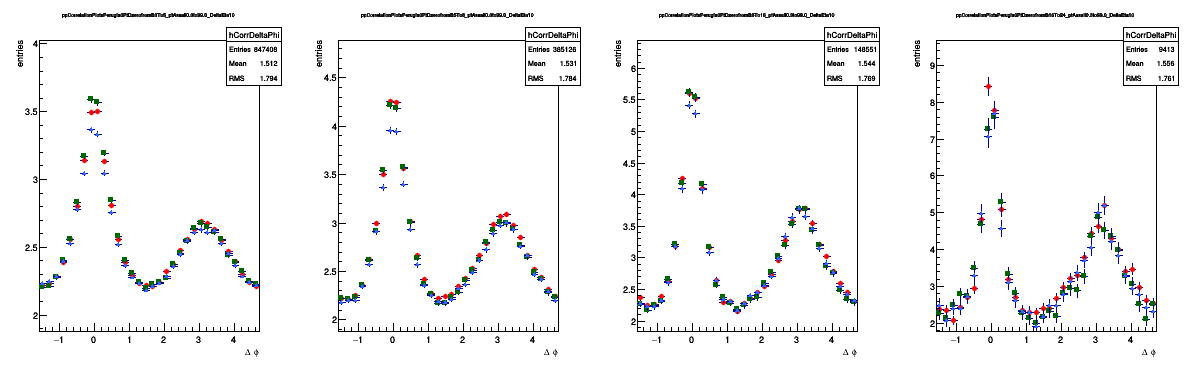
\includegraphics[width=.49\linewidth]{figures/Template/1DCompare_allDpTfromB_AssoPt_0.3to99.0GeVc_Perugia0.png}
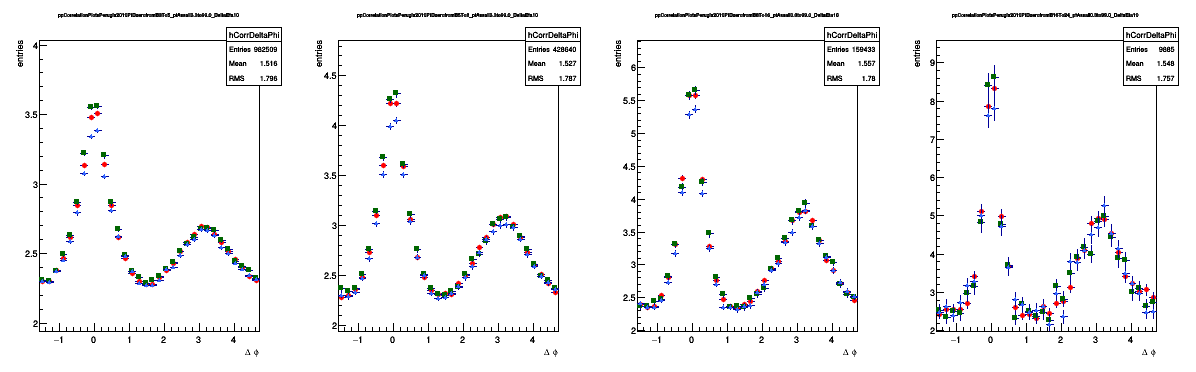
\includegraphics[width=.49\linewidth]{figures/Template/1DCompare_allDpTfromB_AssoPt_0.3to99.0GeVc_Perugia2010.png}
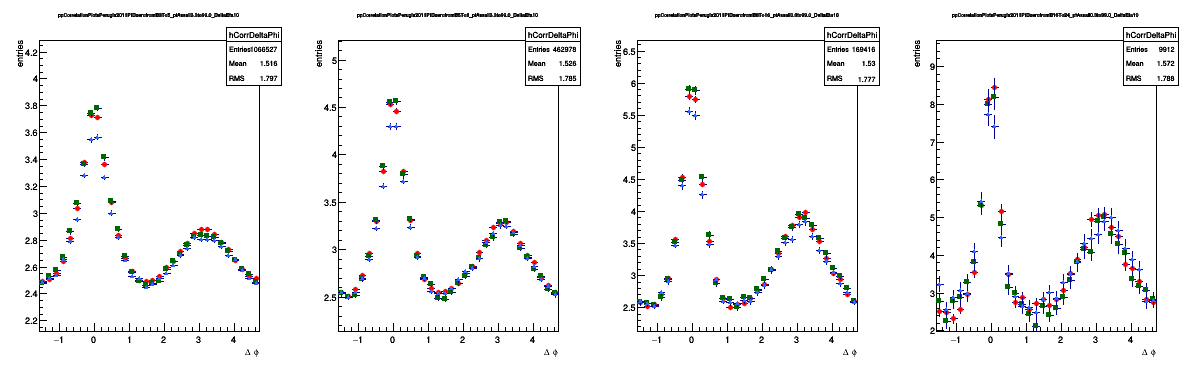
\includegraphics[width=.49\linewidth]{figures/Template/1DCompare_allDpTfromB_AssoPt_0.3to99.0GeVc_Perugia2011.png}
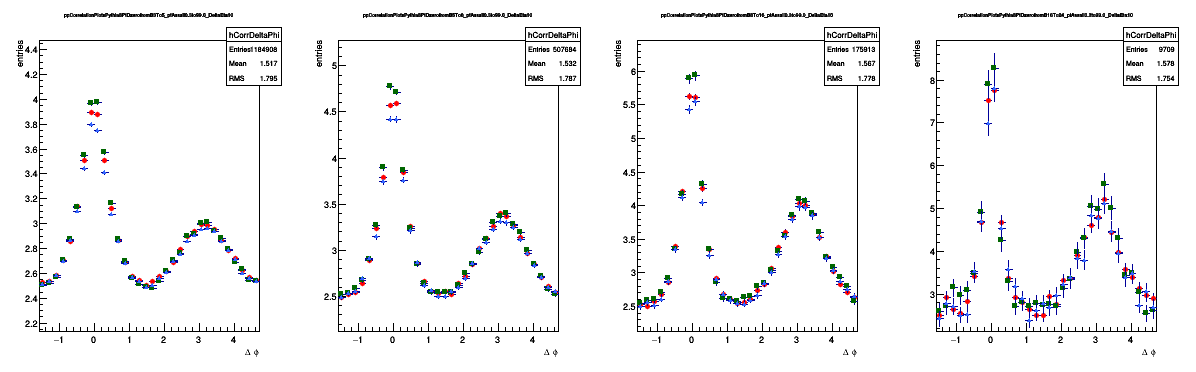
\includegraphics[width=.49\linewidth]{figures/Template/1DCompare_allDpTfromB_AssoPt_0.3to99.0GeVc_Pythia8.png}
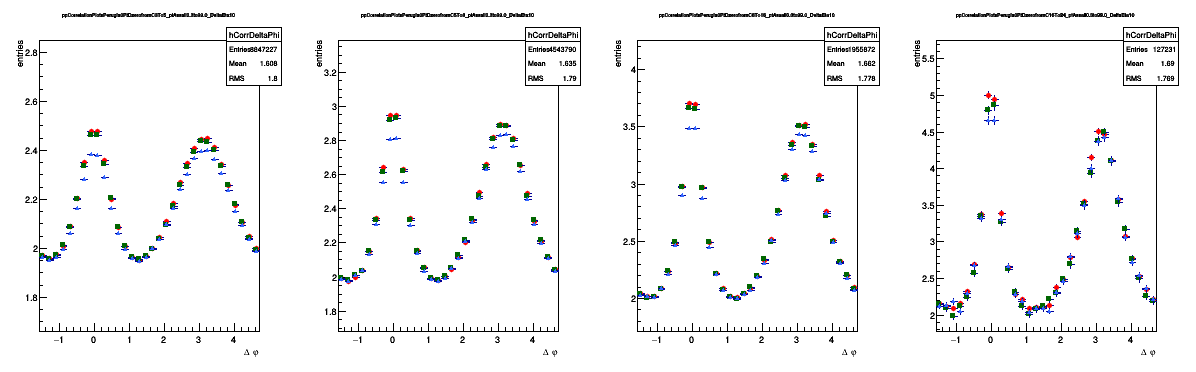
\includegraphics[width=.49\linewidth]{figures/Template/1DCompare_allDpTfromC_AssoPt_0.3to99.0GeVc_Perugia0.png}
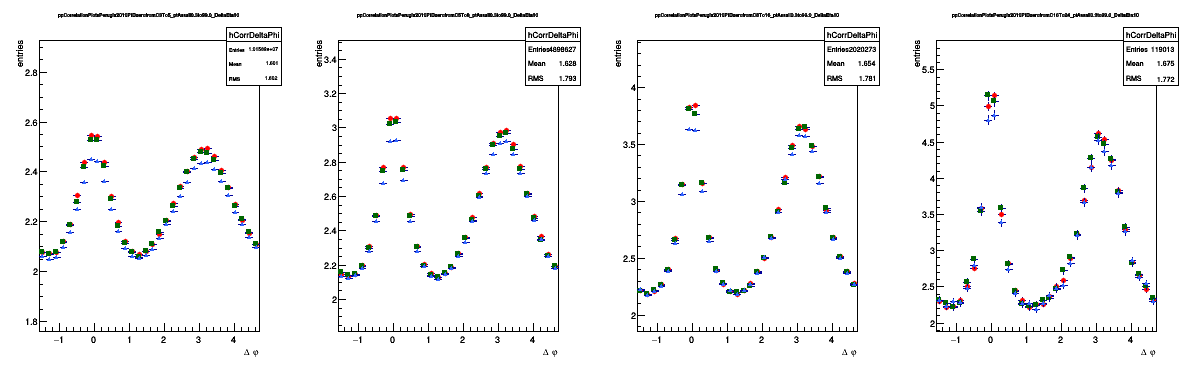
\includegraphics[width=.49\linewidth]{figures/Template/1DCompare_allDpTfromC_AssoPt_0.3to99.0GeVc_Perugia2010.png}
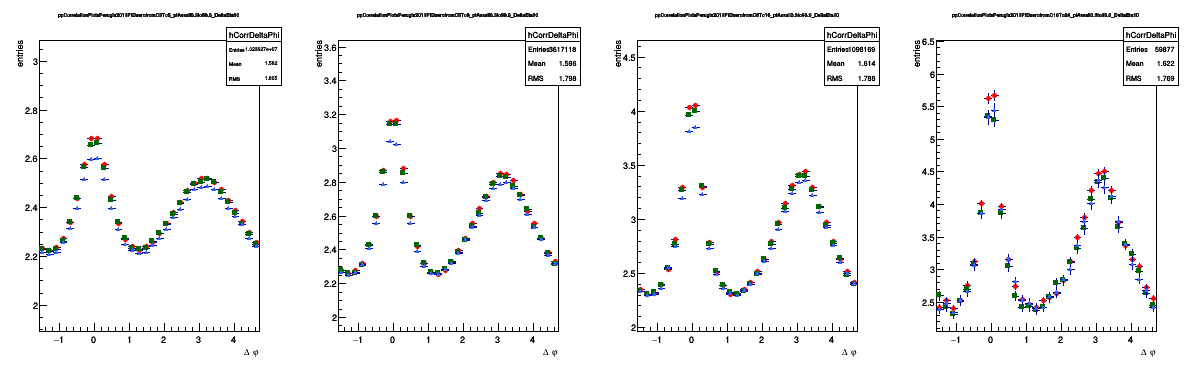
\includegraphics[width=.49\linewidth]{figures/Template/1DCompare_allDpTfromC_AssoPt_0.3to99.0GeVc_Perugia2011.png}
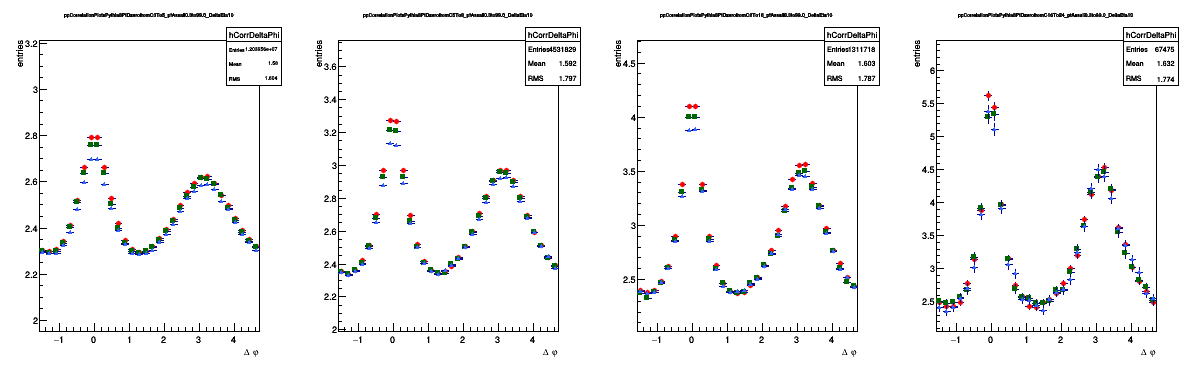
\includegraphics[width=.49\linewidth]{figures/Template/1DCompare_allDpTfromC_AssoPt_0.3to99.0GeVc_Pythia8.png}
\caption{Top left: azimuthal correlation distribution between D meson from b-hadron decay and charged particles obtained from a Monte Carlo simulation
based on Pythia (Perugia-0 tune) fitted with a 2+1 Gaussian + constant function. The violet histogram is the template obtained by scaling the baseline
in order to match that measured in data. Top right: data correlation distributions obtained after the subtraction of the feed-down component, using 3 different values of $f_{\rm prompt}$ resulting
from the variation of the charm and beauty quark masses and factorization and renormalization scales employed in the FONLL calculation. Bottom: ratios between the azimuthal
distribution obtained with the maximum and minimum $f_{\rm prompt}$ values and that obtained with the central $f_{\rm prompt}$ value.}
\label{templates}
\end{figure}

 %The green histogram in figure~\ref{fig:feeddownDescription}, top left panel, represents
%the azimuthal correlation distribution between D meson from b-hadron decay and charged particles obtained from a Monte Carlo simulation
%based on Pythia (Perugia-0 tune). This distribution is
%fitted with a function composed of 2 Gaussian, modeling the near-side peak, 1 Gaussian modeling the away-side peak and a constant term modeling
%the baseline. A second template (violet histogram) is obtained after rescaling the baseline to the value obtained from a fit to the data distribution. In the top right panel
%the data correlation distributions obtained after the subtraction of the feed-down component, using 3 different values of $f_{\rm prompt}$ resulting
%from the variation of the charm and beauty quark masses and factorization and renormalization scales employed in the FONLL calculation, are compared
%to the uncorrected one. As clearly visible the difference is minimal, within few percent. In the bottom panel of the same figure the ratios between the azimuthal
%distribution obtained with the maximum and minimum $f_{\rm prompt}$ values  and that obtained with the central $f_{\rm prompt}$ value show that the uncertainty
%on the feed-down subtraction arising from the uncertainty on the FONLL calculation is contained within 2-3\%. {\bf THE ESTIMATE OF THE UNCERTAINTY DERIVING
%FROM THE MONTE CARLO SIMULATION FROM WHICH THE TEMPLATE IS OBTAINED IS BEING STUDIED.}.

\newpage % always start next (sub)section with new page to avoid disarrangement. 
